\chapter{Phương pháp đề xuất}
\label{Chapter4}  

Trong phần này, chúng tôi trình bày framework MSKGen cho bài toán suy luận đồ thị tri thức thời gian. Mục 4.1 giới thiệu quá trình Trích xuất sự kiện dựa trên luật (Rule-based Facts Extraction), tạo và tinh chỉnh các luật thời gian lặp đi lặp lại bằng LLMs đồng thời trích xuất các sự kiện từ các luật đã tinh chỉnh. Mục 4.2 mô tả cơ chế Truy xuất sự kiện ngữ nghĩa (Semantic Facts Retrieval) sử dụng RAG để thu thập các sự kiện tương đồng ngữ nghĩa, sự kiện tương đồng chủ thể và sự kiện chân lý nền từ cơ sở dữ liệu vector. Mục 4.3 giải thích cơ chế Suy luận đa nguồn (Multi-Source Reasoning) nơi các sự kiện được trích xuất và truy xuất được kết hợp để lý luận theo truy vấn cụ thể bằng LLMs. Cuối cùng, Mục 4.4 chi tiết cơ chế Tính điểm ứng viên (Candidate Scoring) tích hợp các ứng viên do LLM tạo ra với dự đoán từ mô hình đồ thị để xếp hạng và lựa chọn câu trả lời chính xác nhất cho mỗi truy vấn.

\begin{figure}[!htbp]
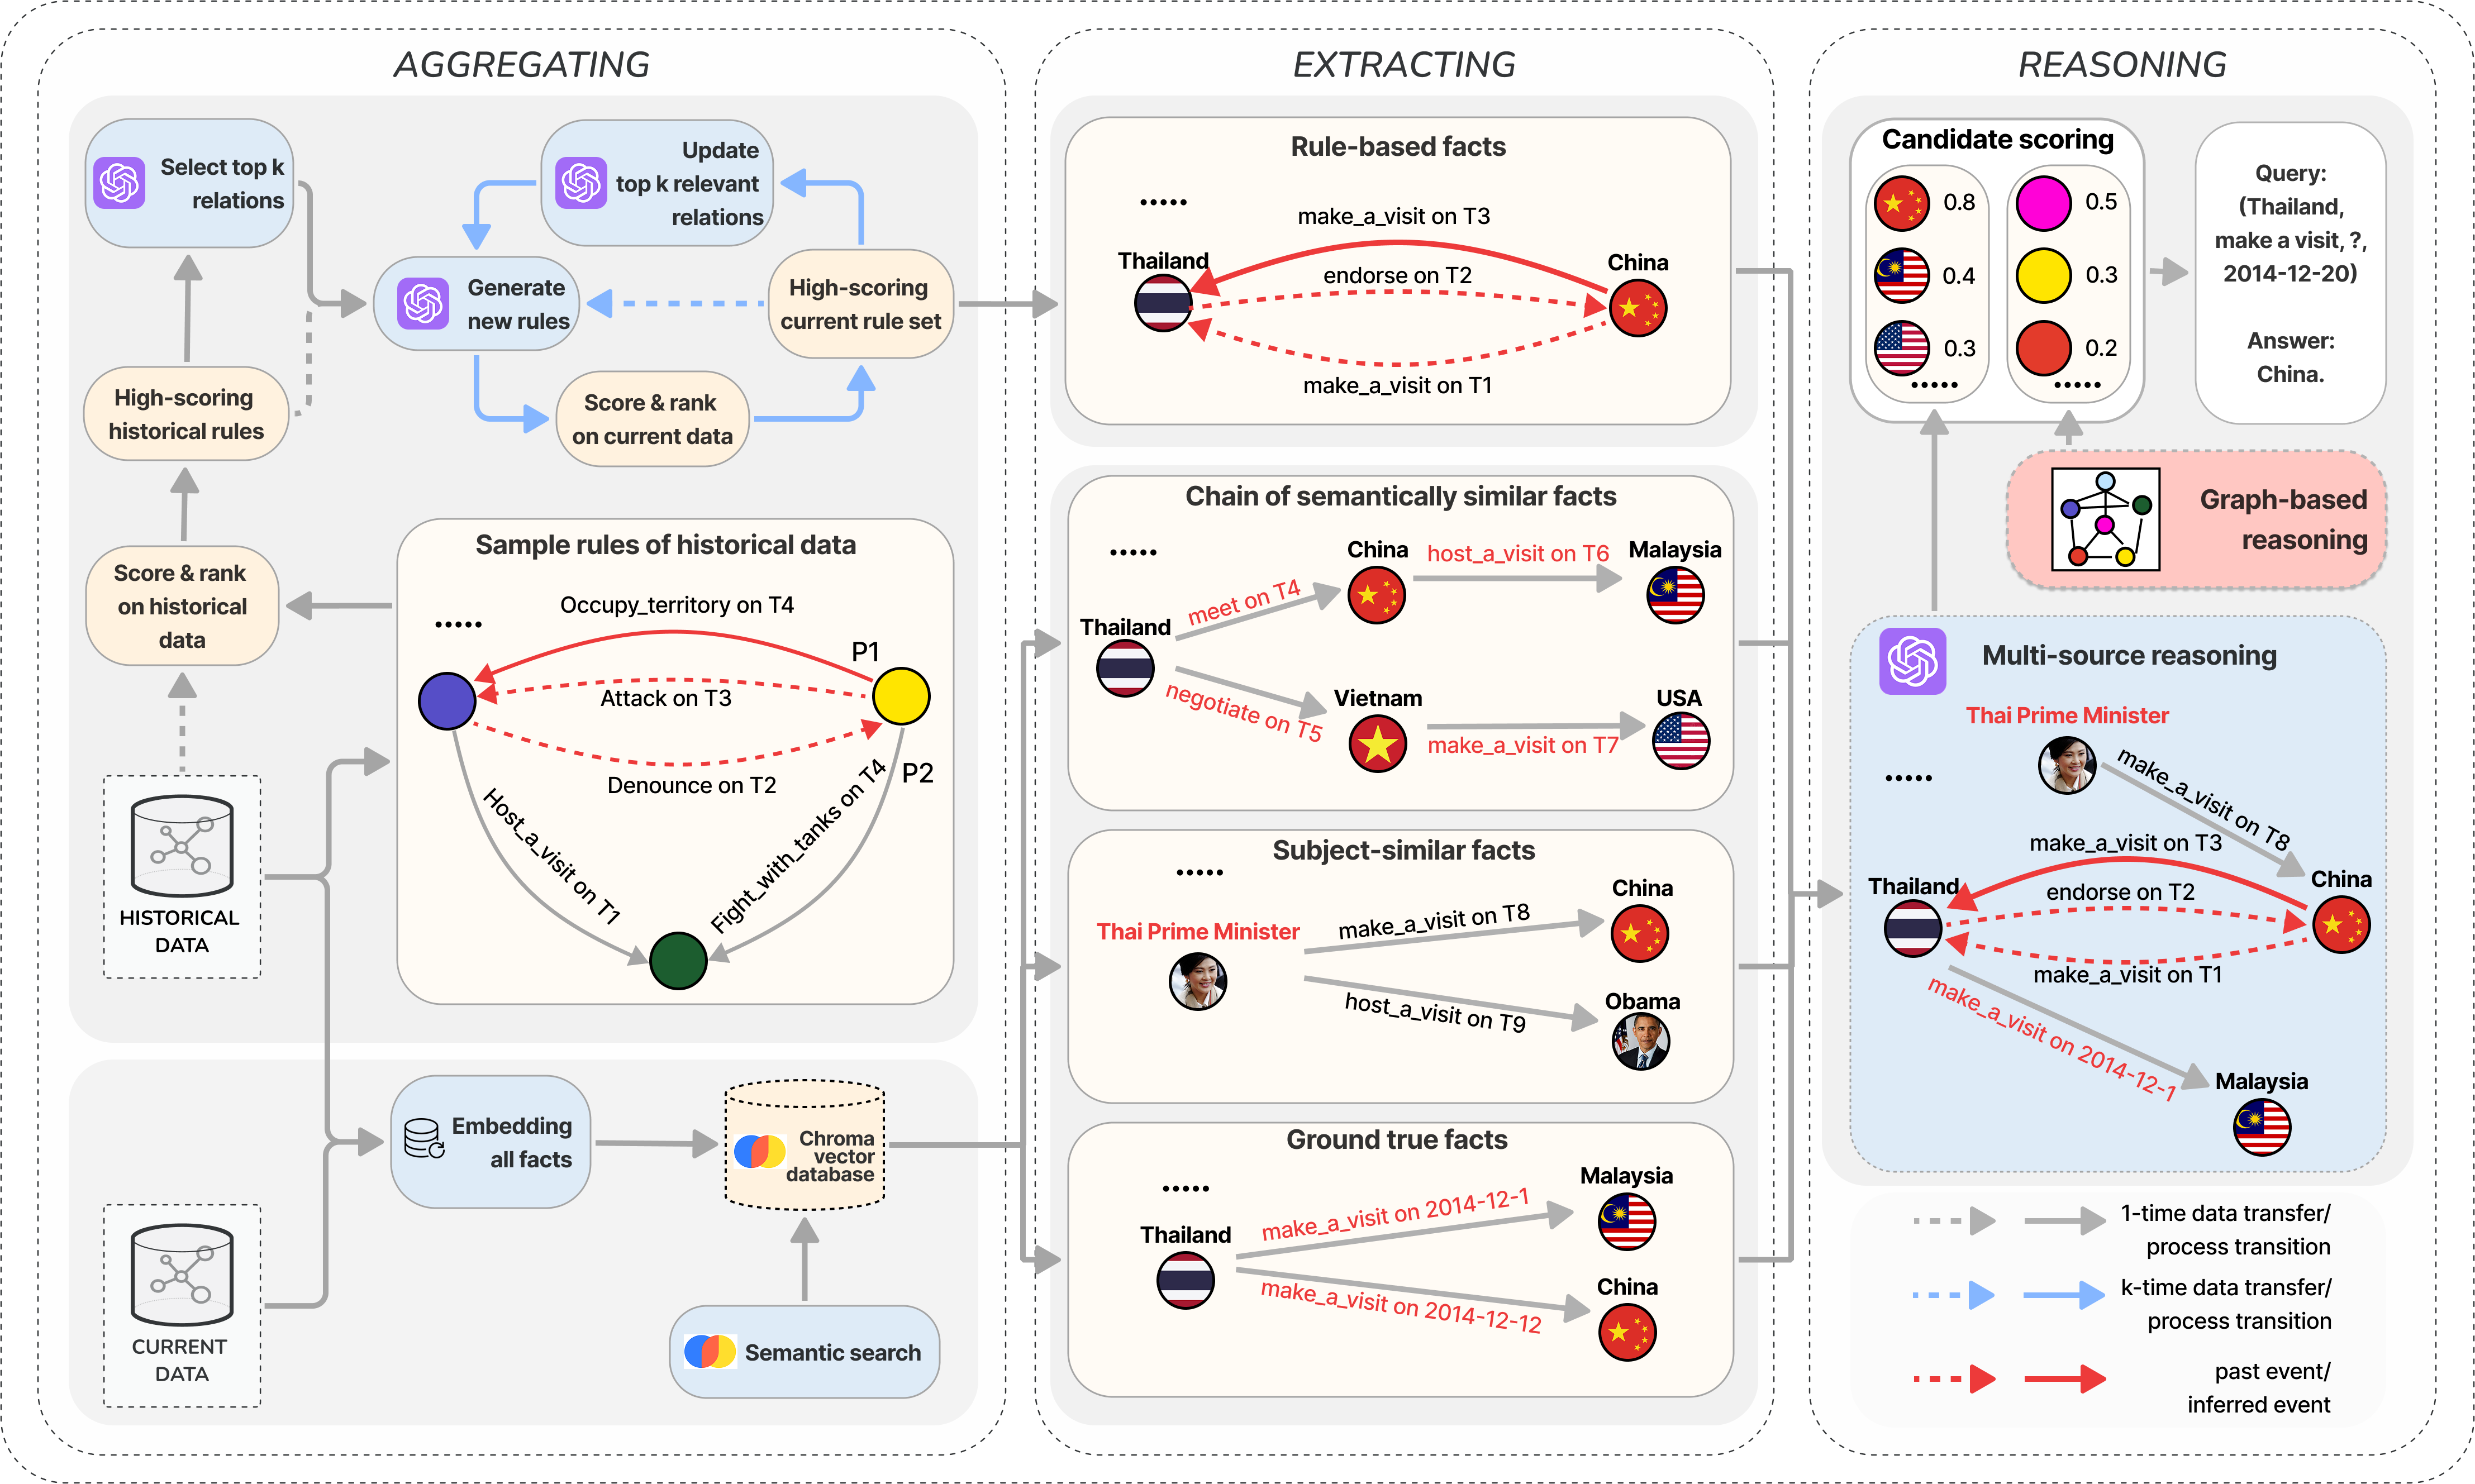
\includegraphics[width=15cm]{images/Framework01.png}
% \includesvg[width=\textwidth]{images/Framework01.svg}
\caption{MSKGen bắt đầu với hai quá trình song song: Trích xuất sự kiện dựa trên luật (Rule-based Facts Extraction) liên tục sử dụng LLMs để tạo luật từ các luật lịch sử được lấy mẫu, tinh chỉnh lặp đi lặp lại các luật mới dựa trên đánh giá từ dữ liệu hiện tại, và trích xuất các sự kiện chất lượng cao từ các luật đã tinh chỉnh; và Truy xuất sự kiện ngữ nghĩa (Semantic Facts Retrieval) nhúng các sự kiện vào cơ sở dữ liệu vector và truy xuất các sự kiện tương đồng ngữ nghĩa, sự kiện tương đồng chủ thể, và sự kiện chân lý nền sử dụng khái niệm RAG. Các sự kiện này được kết hợp trong Suy luận đa nguồn (Multi-Source Reasoning), nơi LLMs tổng hợp câu trả lời đặc thù cho truy vấn bằng cách tích hợp thông tin đa dạng và đồng bộ về mặt ngữ nghĩa.} 
\label{fig1}
\end{figure}

\section{Trích xuất sự kiện dựa trên luật}

\subsection{Trích xuất các luật lịch sử điểm cao và các quan hệ liên quan top k}

\paragraph{Lấy mẫu luật lịch sử.}
Giai đoạn đầu tiên của quá trình trích xuất sự kiện dựa trên luật (Rule-based Facts Extraction) bao gồm việc xác định các luật logic thời gian từ dữ liệu lịch sử bằng phương pháp duyệt ngẫu nhiên có thời gian (temporal random walk). Quá trình lấy mẫu tuân theo các bước chính sau. Đầu tiên, với một luật có độ dài \( l \), một chuỗi duyệt có độ dài \( l+1 \) được lấy mẫu, trong đó bước bổ sung tương ứng với phần đầu luật (rule head). Ở bước lấy mẫu đầu tiên \( m = 1 \), một cạnh \( (e_1, r_h, e_{l+1}, t_{l+1}) \) được lấy mẫu đồng nhất từ tất cả các cạnh có loại quan hệ \( r_h \). Bộ duyệt ngẫu nhiên thời gian sau đó lặp lại việc lấy mẫu các cạnh kề với đối tượng hiện tại cho đến khi thu được một chuỗi duyệt có độ dài \( l+1 \).

Để duy trì tính nhất quán thời gian, quá trình lấy mẫu sử dụng hàm xác suất chuyển tiếp (\ref{eq2}):
\begin{equation}
    \label{eq2}
    P(u; m, e_m, t_m) = \frac{\exp(t_u - t_m)}{\sum_{u' \in A(m, e_m, t_m)} \exp(t_{u'} - t_m)}
\end{equation}
nơi các cạnh gần thời gian hơn với nút hiện tại có xác suất lấy mẫu cao hơn. Điều này đảm bảo thứ tự thời gian được bảo toàn trong suốt quá trình duyệt và các sự kiện tương lai không thể ảnh hưởng đến sự kiện quá khứ. Cuối cùng, các chuỗi duyệt được lấy mẫu được chuyển đổi thành các luật bằng cách thay thế các thực thể thành biến số trong khi duy trì tham chiếu thực thể và bảo toàn các ràng buộc thời gian giữa các sự kiện.

\paragraph{Đánh giá chất lượng luật.}
Sau khi thu được các luật mẫu từ dữ liệu lịch sử thông qua duyệt ngẫu nhiên thời gian, chúng tôi triển khai quá trình trích xuất để xác thực chất lượng luật và tạo ra các quan hệ liên quan. Các luật mẫu trải qua quá trình đánh giá chất lượng sử dụng thước đo Kulczynski \cite{ref_article16} trên dữ liệu lịch sử, được định nghĩa (\ref{eq3}):
\begin{equation}
\label{eq3}
    Kulczynski(R) = \frac{1}{2} \left( \frac{r}{r_b} + \frac{r}{r_h} \right)
\end{equation}
trong đó: \( r_b \) biểu thị số cặp sự kiện thời gian thỏa mãn thân luật (rule body), \( r_h \) biểu thị số cặp sự kiện thời gian thỏa mãn đầu luật (rule head), \( r \) biểu thị số cặp sự kiện thỏa mãn cả điều kiện thân luật và đầu luật. Các luật vượt ngưỡng \( \gamma \) được phân loại là luật điểm cao.

\textit{Quá trình lựa chọn quan hệ.} Sau đánh giá chất lượng luật, với mỗi quan hệ trong dữ liệu hiện tại, chúng tôi triển khai quá trình lựa chọn quan hệ để xác định top-$k$ quan hệ liên quan nhất cho việc xây dựng luật thời gian. Quá trình này tận dụng Large Language Models (LLMs) thông qua phương pháp nhắc có cấu trúc. \textbf{User Message} chứa đầu vào biến đổi đặc thù cho từng truy vấn (đầu luật, các luật điểm cao, và các quan hệ khả dụng), trong khi \textbf{System Message} cung cấp hướng dẫn nhất quán xuyên suốt tất cả các trường hợp nhắc.


\begin{promptbox}{Prompt lựa chọn quan hệ liên quan}
\textbf{User Message:}
Cho trước một quan hệ đầu luật mục tiêu, hãy phân tích các luật điểm cao và các quan hệ khả dụng để xác định top-$k$ quan hệ liên quan nhất có thể tạo thành các luật thời gian có ý nghĩa.
\begin{itemize}
    \item \textbf{Đầu luật:} \texttt{\{rule\_head\}} - Quan hệ mục tiêu cho việc sinh luật
    \item \textbf{Tổ hợp logic hiện tại:} \texttt{\{high\_scoring\_rules\}} - Các luật điểm cao từ đánh giá luật
    \item \textbf{Quan hệ khả dụng:} \texttt{\{relation\_list\}} - Các quan hệ ứng viên để xây dựng luật
\end{itemize}

\textbf{System Message:} Chọn các quan hệ ứng viên thỏa mãn: Có liên kết ngữ nghĩa mạnh với quan hệ đầu luật, thể hiện khả năng dự đoán cao dựa trên các mẫu dữ liệu lịch sử và có thể tạo thành các luật thời gian có ý nghĩa khi kết hợp.
\end{promptbox}

\subsection{Sinh luật và tinh chỉnh lặp}

\paragraph{Sinh luật mới.}
Quá trình tạo các luật thời gian mới tận dụng Large Language Models (LLMs) thông qua phương pháp nhắc có cấu trúc. Cách tiếp cận này sử dụng các luật lịch sử điểm cao và các quan hệ liên quan top-k làm đầu vào. Chiến lược nhắc được thiết kế để hướng dẫn LLM tạo ra các luật logic thời gian toàn diện và có ý nghĩa....
\begin{promptbox}{Prompt sinh luật mới}
\textbf{User Message:}
Sinh các luật logic thời gian cho quan hệ mục tiêu thông qua Suy luận từng bước.
\begin{itemize}
    \item \textbf{Quan hệ mục tiêu:} \texttt{\{head\_relation\}(X, Y, T)} - Quan hệ mục tiêu cho việc sinh luật
    \item \textbf{Luật tham chiếu:} \texttt{\{high\_scoring\_rules\}} - Các luật tham chiếu điểm cao
    \item \textbf{Quan hệ ứng viên được cung cấp:} \texttt{\{relevant\_relations\}} - Các quan hệ ứng viên được cung cấp
\end{itemize}

\textbf{System Message:} Sử dụng các quan hệ từ phần thân của các luật tham chiếu và các quan hệ ứng viên được cung cấp, đảm bảo mỗi luật được sinh ra: duy trì tính nhất quán thời gian, tạo ra các liên kết ngữ nghĩa có ý nghĩa và hình thành các đường dẫn suy luận thời gian hợp lệ.\\
Ví dụ:

\begin{itemize}
    \item \textbf{Quan hệ mục tiêu:} Make a visit(X0, X1, T)
    \item \textbf{Luật tham chiếu:}
    \begin{itemize}
        \item Make a visit(X0, X1, T) $\leftarrow$ Host a visit(X1, X0, T0)
        \item Make a visit(X0, X2, T3) $\leftarrow$ Consult(X0, X1, T0)
    \end{itemize}
    \item \textbf{Quan hệ ứng viên được cung cấp:} Praise or endorse(X0, X1, T), Plan to meet(X0, X1, T), Engage in negotiation(X0, X1, T)
    $\Rightarrow$ \textbf{Luật sinh ra:} Make a visit(X0, X1, T3) $\leftarrow$ Endorse(X0, X1, T0) $\land$ Plan to meet(X1, X0, T1) $\land$ Host a visit(X0, X1, T2)
\end{itemize}
\end{promptbox}


\paragraph{Đánh giá và xếp hạng luật.}
Các luật được tạo ra trải qua đánh giá chất lượng sử dụng thước đo Kulczynski để so sánh chất lượng giữa các luật trong tập Generated rules dựa trên việc đánh giá chúng trên dữ liệu hiện tại. Thước đo Kulczynski, như đã định nghĩa trước đó, được sử dụng để đánh giá chất lượng luật. Các luật vượt ngưỡng $\gamma$ được thêm vào tập luật dưới dạng các luật hiện tại điểm cao. Quá trình đánh giá này đảm bảo chỉ các luật có độ chính xác và phạm vi bao phủ đủ tiêu chuẩn được giữ lại để sử dụng tiếp trong quá trình suy luận đồ thị tri thức thời gian.

\paragraph{Tinh chỉnh tập quan hệ liên quan: Cập nhật tập quan hệ liên quan Top k của mỗi đầu luật.}
Với mỗi đầu luật, chúng tôi đánh giá chất lượng quan hệ thông qua phép tính tỷ lệ (\ref{eq4}):
\begin{equation}
    \label{eq4}
    Quality(rel_i) = \frac{N_{high}(rel_i)}{N_{total}(rel_i)}
\end{equation}

trong đó $N_{high}(rel_i)$ biểu thị số lượng luật điểm cao chứa quan hệ $i$, và $N_{total}(rel_i)$ biểu thị tổng số luật được tạo ra chứa quan hệ $i$. Quá trình tinh chỉnh xác định $n$ quan hệ cuối (trong số $k$) dựa trên điểm chất lượng và cập nhật chúng thông qua lựa chọn có hướng dẫn bởi LLM:

\begin{promptbox}{Prompt tinh chỉnh tập quan hệ liên quan}
\textbf{User Message:}
Cho trước một đầu luật và các quan hệ hiệu suất thấp của nó, phân tích các luật điểm cao và các quan hệ khả dụng để xác định các quan hệ thay thế có thể nâng cao chất lượng luật thời gian.
\begin{itemize}
    \item \textbf{Đầu luật:} \texttt{\{rule\_head\}} - Quan hệ mục tiêu cho việc sinh luật
    \item \textbf{Tổ hợp logic hiện tại:} \texttt{\{high\_scoring\_rules\}} - Các luật điểm cao từ đánh giá luật
    \item \textbf{Quan hệ hiệu suất thấp:} \texttt{\{low\_quality\_relations\}} - Các quan hệ cần thay thế
    \item \textbf{Quan hệ khả dụng:} \texttt{\{relation\_list\}} - Các quan hệ ứng viên để thay thế
\end{itemize}

\textbf{System Message:} Lựa chọn các quan hệ thay thế có: Kết nối ngữ nghĩa mạnh với đầu luật và thể hiện khả năng dự đoán cao dựa trên các tổ hợp logic hiện tại.
\end{promptbox}

\paragraph{Cải tiến lặp.}
Toàn bộ quá trình hoạt động theo chu kỳ liên tục, nơi các luật mới được tạo ra bằng cách sử dụng các quan hệ đã cập nhật và các luật điểm cao mới, sau đó tiến hành đánh giá chất lượng và tinh chỉnh quan hệ. Quá trình này tiếp tục cho đến khi tập luật đạt được số lần lặp xác định trước, cuối cùng tạo ra tập luật hoàn thiện.

\subsection{Trích xuất sự kiện dựa trên luật}

\paragraph{Quá trình trích xuất sự kiện dựa trên luật.}
Với một truy vấn $q = (e_s, r, ?, t_q)$, chúng tôi lọc các luật từ tập luật hiện tại điểm cao nơi đầu luật khớp với $r$. Chúng tôi sau đó cụ thể hóa các luật này bằng cách thay thế thực thể truy vấn $e_s$ vào vị trí thích hợp, duy trì ràng buộc thời gian. Bằng cách tìm kiếm trong dữ liệu hiện tại các mẫu sự kiện phù hợp thỏa mãn thân luật $\bigwedge_{i=1}^{l-1} r_i(e_s, e_o, t_i)$, chúng tôi trích xuất các sự kiện dựa trên luật hoàn chỉnh tạo thành các chuỗi lý luận nhất quán thời gian để dự đoán các câu trả lời tiềm năng.

\vspace{1em}
\section{Trích xuất sự kiện theo ngữ nghĩa}

Phương pháp trích xuất sự kiện thứ hai mà MSKGen sử dụng là phương pháp trích xuất dựa theo ngữ nghĩa sử dụng ý tưởng của RAG để giải quyết bài toán suy luận trên đồ thị tri thức theo thời gian. Không giống các phương pháp truy xuất "khô cứng" mà chỉ phụ thuộc hoàn toàn vào việc làm khớp các lược đồ/từ khóa (schema matching) một cách chính xác, phương pháp này sử dụng các vector nhúng tiềm ẩn để nắm bắt sự tương đồng về ngữ nghĩa giữa các chủ thể, sự kiện. Điều này giúp mở rộng không gian tìm kiếm và cung cấp ngữ cảnh phong phú hơn cho mô hình ngữ ngôn lớn trong quá trình suy luận.

\vspace{1em}
\subsection{Tiền xử lý dữ liệu}
Để chuẩn bị cho giai đoạn truy xuất, MSKGen sẽ thực hiện tiền xử lý và nhúng tất cả các sự kiện (fact) vào một cơ sở dữ liệu chung gọi là cơ sở dữ liệu vector.

MSKGen bắt đầu bắt việc chuyển đổi tất cả các sự kiện từ định dạng văn bản có cấu trúc gồm bốn thành phần ($s, r, o, t$) thành một câu hoàn chỉnh diễn tả đầy đủ nội dung sự kiện được ngụ ý bởi bốn thành phần này. Ví dụ bộ bốn (\textit{Malaysia, make\_a\_visit, Thailand, 2014-9-12}) sẽ được chuyển thành một câu hoàn chỉnh \textit{Malaysia made a visit to Thailand on 2014-9-12}. Quy trình này đảm bảo thông tin ngữ nghĩa và bối cảnh của mỗi sự kiện sẽ được giữ nguyên khi nhúng sang không gian vector.

Để trích xuất tri thức ẩn chứa trong mỗi fact, MSKGen sử dụng kĩ thuật nhúng (embedding) để chuyển văn bản thành các vector đặc trưng. Trong quá trình này, \textbf{Chroma} được chọn làm cơ sở dữ liệu vector vì đây là một hệ thống lưu trữ chuyên dụng, được thiết kế cho việc lưu trữ và truy vấn các vector nhúng với hiệu suất cao. Bằng cách sử dụng tính năng tìm kiếm theo độ tương đồng cosine của Chroma, các sự kiện có nội dung tương đồng về ngữ nghĩa với sự kiện truy vấn có thể được truy xuất một cách chính xác ngay cả khi giữa chúng không có sự trùng khớp về từ khóa.

\vspace{1em}
\subsection{Xây dựng cơ sở dữ liệu vector}

Cơ sở dữ liệu trong MSKGen được thiết kế để không chỉ đơn giản là một hệ thống lưu trữ vector nâng cao mà còn cung cấp một cấu trúc lưu trữ tài liệu linh hoạt. Cụ thể, mỗi sự kiện sẽ được chuyển đổi thành một tài liệu (document) với ba thành phần chính:
\begin{itemize}
    \item \textbf{Metadata:} Thành phần này đóng vai trò như một bộ lọc (filter) trước khi quá trình tìm kiếm tài liệu được thực hiện. Metadata của mỗi tài liệu được thiết kế dưới dạng một từ điển (dictionary) $\mathcal{M} = \{\mathcal{S, R, E, T}\}$, trong đó $\mathcal{S, R, E, T}$ lần lượt là thực thể chủ ngữ, mối quan hệ giữa 2 thực thể trong sự kiện, thực thể vị ngữ và mốc thời gian. Cách thiết kế này giúp lọc ra các tài liệu khônng muốn, thu hẹp không gian tìm kiếm, đồng thời nâng cao cả độ chính xác lẫn tốc độ tìm kiếm.
    \item \textbf{Nội dung trang (page content):} Đây là chuỗi văn bản mô tả sự kiện có được sau giai đoạn tiền xử lý. Thành phần này sẽ được nhúng thành vector và vector đó sẽ được dùng để so sánh sự tương đồng với vector của truy vấn.
    \item \textbf{Vector nhúng (vector embedding):} Đây là vector số biểu diễn cho nội dung trang của tài liệu sau khi đã được nhúng. Việc chuyển đổi nội dung trang sang vector nhúng được thực hiện bởi mô hình nhúng được huấn luyện sẵn của OpenAI - \textbf{text-embedding-3-large} \cite{ref_article18}.
\end{itemize}

\vspace{1em}
\subsection{Phương pháp truy xuất ngữ nghĩa}

Với truy vấn $\mathcal{Q}$, MSKGen sẽ trích xuất ra ba thành phần - chủ thể $\mathcal{S}$, quan hệ $\mathcal{R}$ và mốc thời gian $\mathcal{T}$ - để hỗ trợ quá trình truy xuất. Để truy xuất các sự kiện mà chủ thể hoặc quan hệ của nó có ngữ nghĩa tương tự với $\mathcal{S, R}$ thông qua cơ sở dữ liệu vector. Đầu tiên, MSKGen sử dụng bộ lọc metadata để giảm không gian tìm kiếm. Sau khi đã loại bỏ bớt các tài liệu không cần thiết, MSKGen sẽ tiếp tục việc tìm kiếm trên các tài liệu còn lại. Cụ thể, tùy vào chiến lược truy xuất thì chủ thể $\mathcal{S}$ hoặc quan hệ $\mathcal{R}$ sẽ được nhúng thành vector truy vấn $\mathcal{Q}$ bằng cách sử dụng mô hình text-embedding-3-large (\ref{eq:query-embed}):
\begin{equation}  
\label{eq:query-embed}  
Q = \text{text-embedding-3-large}(\mathcal{R}). 
\end{equation}

Sau đó, MSKGen sẽ truy xuất top k tài liệu mà vector nhúng của nội dung trang có sự tương đồng về mặt ngữ nghĩa nhất với vector truy vấn $\mathcal{Q}$ dựa trên độ đo tương đồng cosine (\ref{eq:cos-sim_1},\ref{eq:top-sim_2}):
\begin{equation}  
\label{eq:cos-sim_1}  
\text{Cos-Sim}(Q, d_{i})   
\,=\, \frac{Q \cdot d_{i}}{\|Q\|\;\|d_{i}\|}  
\end{equation}

\begin{equation}  
\label{eq:top-sim_2}  
\text{Top-}k   
= \arg\max_{d_i \in D}^{k}\,\text{Cos-Sim}(Q, d_i).    
\end{equation} 

Trong đó $\cdot$ là phép nhân vô hướng, $\|\cdot\|$ biểu diễn chuẩn (norm) của vector, $d_{i}$ kí hiệu vector nhúng của tài liệu thứ $i$ và $\text{Top-}k$ là tập hợp $k$ tài liệu mà nội dung trang của chúng có sự tương đồng về mặt ngữ nghĩa với truy vấn nhất.

\vspace{1em}
\subsection{Chiến lược truy xuất sự kiện}

Dự đoán của các mô hình ngôn ngữ lớn phụ thuộc rất nhiều vào ngữ cảnh được cung cấp. Việc chỉ truy xuất các sự kiện khớp cứng với từ khóa cho trước (ICL) hoặc các sự kiện dạng chuỗi lịch sử (CoH) sẽ bỏ qua những kết nối ngữ nghĩa quan trọng. Chẳng hạn, các quyết định hợp tác của Malaysia có thể chịu ảnh hưởng không chỉ bởi các đối tác trước đây mà còn bởi các sự kiện khác như việc viếng thăm hoặc những cuộc họp quan trọng. Vì vậy đối với một truy vấn dạng bộ bốn $\mathcal{Q = (S, R, ?, T})$, MSKGen thực hiện chiến lược truy xuất cho ba tập hợp sự kiện sau:
\begin{itemize}
    \item \textbf{Chuỗi các sự kiện tương đồng về mặt ngữ nghĩa:} Đây là một chuỗi các sự kiện bắt đầu từ chủ thể $\mathcal{S}$ và có quan hệ tương đồng về mặt ngữ nghĩa với quan hệ $\mathcal{R}$. Các chuỗi sự kiện này sẽ được lưu vào một tập hợp, kí hiệu là $H_C$. Tập $H_C$ sẽ giúp LLM thực hiện suy luận đa bước (multi-hop reasoning), do đó các sự kiện trong $H_C$ sẽ được sắp xếp theo thứ tự tăng dần của thời gian.
    \item \textbf{Các sự kiện có chủ thể tương đồng với chủ thể truy vấn:} Một hạn chế lớn thường bị bỏ qua là khi chủ thể $\mathcal{S}$ trong truy vấn hoàn toàn mới và không có dữ liệu lịch sử, khiến LLM thiếu thông tin để suy luận. Để khắc phục điều này, MSKGen thay thế $\mathcal{S}$ bằng các thực thể tương tự có các mối quan hệ liên quan. Nếu không có sự kiện lịch sử nào liên quan tới $\mathcal{S}$, LLM sẽ sử dụng các sự kiện từ các thực thể tương tự này vì chúng thường chia sẻ những hình hành vi chung. Các sự kiện này được lưu trong tập $H_S$ và sẽ được dùng để bổ sung ngữ cảnh cho LLM, đặc biệt khi tập $H_C$ không đủ hoặc bị thiếu.
    \item \textbf{Ground true của những sự kiện tương tự vừa xảy ra trước truy vấn $\mathcal{Q}$:} Để tránh việc LLM liên tục trả lời sai đối với các truy vấn cùng chủ thể $\mathcal{S}$ và quan hệ $\mathcal{R}$ và có mốc thời gian gần nhau, MSKGen sẽ cung cấp thêm cho LLM các ground true của những sự kiện tương tự vừa xảy ra trước sự kiện truy vấn $\mathcal{Q}$. Những sự kiện này sẽ được lưu vào tập $H_G$.
\end{itemize}

Việc lưu trữ các sự kiện được truy xuất vào 3 tập khác nhau $H_C, H_S$ và $H_G$ là không khả thi vì sẽ tiêu tốn quá nhiều token đầu vào dẫn đến có thể vượt quá độ dài ngữ cảnh mà mô hình ngôn ngữ lớn cho phép. Do đó, MSKGen giới hạn các tập này chỉ còn các sự kiện phù hợp nhất, cụ thể là các sự kiện lịch sử từ quá khứ xa và gần. Chiến lược lựa chọn này giúp duy trì các mối liên hệ lâu dài và ngắn hạn quan trọng, qua đó nâng cao độ chính xác dự đoán của LLM. 

\vspace{1em}
\section{Suy luận tri thức đa nguồn}
Đối với các truy vấn theo thời gian có dạng $\mathcal{Q = (S, R, ?, T)}$, MSKGen sẽ cung cấp các sự kiện truy xuất dựa trên luật và các sự kiện truy xuất dựa trên ngữ nghĩa cho LLM thông qua User Message và System Message.

System Message chứa một hướng dẫn chi tiết, điều phối quá trình suy luận qua các giai đoạn thao tác rời rạc. Mỗi giai đoạn kết hợp các chỉ dẫn theo ngữ cảnh với ví dụ minh họa cho từng nhóm sự kiện, giúp mô hình tổng hợp dần dần các bằng chứng thời gian trong khi vẫn duy trì mạch suy luận nhất quán. Tất cả các sự kiện được cung cấp cho LLM sẽ được gửi thông qua User Message.

MSKGen giới hạn LLM chỉ trả về $k$ ứng viên có khả năng cao nhất, nhờ vậy giảm bớt việc lãng phí token cho các kết quả kém khả thi. Cuối cùng, MSKGen hợp nhất hai danh sách ứng viên — một từ suy luận dựa trên các sự kiện truy xuất từ luật và một từ suy luận dựa trên các sự kiện truy xuất dựa trên ngữ nghĩa — thành một danh sách ứng viên cuối cùng duy nhất.

\vspace{1em}
\section{Cách tính điểm các ứng viên}

Điểm số cuối cùng của MSKGen trả về bao gồm 2 thành phần chính: điểm số của LLM (LLM-based score) và điểm số lấy từ mô hình đồ thị đã được huấn luyện sẵn (Graph-based score).

\vspace{1em}
\subsection{Điểm số dự đoán của LLM}

Với mỗi thực thể ứng cử viên $c_i$ từ tập ứng cử viên $C$ trả về bởi LLM cho truy vấn $\mathcal{Q}$, MSKGen sẽ tính điểm nó bằng cách kết hợp thứ hạng (rank) của thực thể này được xếp bởi LLM và độ chênh lệch thời gian giữa mốc thời gian $\mathcal{T}$ của truy vấn với mốc thời gian gần nhất mà $c_i$ tương tác với $\mathcal{S}$ (được kí hiệu là $\mathcal{T}_{c_i}$) (\ref{eq:score-llm}):
\begin{equation}  
\label{eq:score-llm}  
\text{score}^{c_i}_{\text{LLM}}   
= \alpha \times \Bigl(1 - \frac{r_{c_i}}{k}\Bigr)  
\;+\; (1 - \alpha)\,\times\, e^{\lambda \,\bigl(\mathcal{T}_{c_i} - \mathcal{T}\bigr)}   
\end{equation}

Trong đó, $\lambda$ biểu thị cho hệ số suy giảm theo thời gian (time decay), $k$ là số lượng ứng cử viên tối đa được LLM trả về và $\alpha$ là trọng số cho dự đoán của LLM. Đối với các thực thể nằm trong tập thực thể của bộ dữ liệu nhưng không có trong dự đoán của LLM thì điểm số của chúng sẽ là 0.

\vspace{1em}
\subsection{Điểm số từ dự đoán của mô hình học sâu theo phương pháp nhúng đồ thị}

Do hạn chế về đầu ra, danh sách ứng viên được tạo ra bởi LLM có thể không có khả năng để khớp với đáp án của toàn bộ câu truy vấn. Để nâng cao độ chính xác của kết quả cuối cùng, MSKGen có tích hợp thêm kết quả của mô hình học sâu theo phương pháp nhúng đồ thị. Điểm số của ứng cử viên $c_i$ có từ mô hình học sâu theo phương pháp nhúng kí hiệu là $\text{score}_G^{c_i}$.

\vspace{1em}
\subsection{Điểm số cuối cùng}

Điểm số cuối cùng của một thực thể ứng cử viên sẽ là sự tổng hợp từ hai điểm số trên (\ref{eq:final-score}):
\begin{equation}
    \label{eq:final-score}
    \text{score}^{c_i} = \alpha \times \text{score}^{c_i}_{\text{LLM}} + (1 - \alpha) \times \text{score}_G^{c_i}
\end{equation}

Trong đó $\alpha$ và $1 - \alpha$ lần lượt kí hiệu cho trọng số dự đoán của LLM và trọng số dự đoán của mô hình học sâu theo phương pháp nhúng.

